\documentclass[11pt,varwidth=\maxdimen]{standalone}
%\documentclass{article}
\usepackage[english]{babel}	
\usepackage[utf8]{inputenc}	% Allows for writing special charachters in the tex-file 

\usepackage{amsfonts,amsmath,amssymb,bm,mathrsfs,mathtools,dsfont} 	% Standard mathematics 


\newcommand{\braces}[1]{\left\lbrace #1 \right\rbrace}
\newcommand{\brackets}[1]{\left( #1 \right)}
\newcommand{\squarebrackets}[1]{\left[ #1 \right]} 
\newcommand{\angles}[1]{\left\langle #1\right\rangle}
\newcommand{\abs}[1]{\left\lvert #1 \right\rvert}
\newcommand{\norm}[1]{\left\Vert #1 \right\Vert}

\usepackage[dvipsnames,table]{xcolor}
\definecolor{rmp}{RGB}{41, 43, 133}
\definecolor{myblue}{rgb}{0.24, 0.36, 0.44}
\definecolor{mygreen}{rgb}{0.367, 0.473, 0.0}
\newcommand{\myBlue}[0]{RoyalBlue}
\newcommand{\myGreen}[0]{OliveGreen}
\newcommand{\myRed}[0]{OrangeRed}
\newcommand{\myYellow}[0]{Goldenrod}


\usepackage{tikz}
\usepackage[compat=1.1.0]{tikz-feynman}
\usetikzlibrary{positioning,shapes,calc,arrows.meta}
\newcommand{\coord}[4]{({(#1)+(#3)*cos(#4)},{(#2)+(#3)*sin(#4)})}


\newcommand{\sscript}[1]{{\scriptscriptstyle \mathrm{#1}}}
\newcommand{\EFT}{\sscript{EFT}}


% % % % % % Commands % % % % % % %

\begin{document}

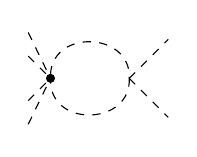
\begin{tikzpicture}[baseline=(a)]
    \begin{feynman}[inline=(a)]
      \vertex[dot] (a) {};
      \vertex[above left=0.4cm of a] (l1);
      \vertex[below left=0.4cm of a] (l2);
      \vertex[above=0.3cm of l1] (l11);
      \vertex[below=0.3cm of l2] (l22);
      \vertex[right=1cm of a] (b);
      \vertex[above right=0.7cm of b] (r1);
      \vertex[below right=0.7cm of b] (r2);
      \diagram*[baseline=(a.base)] {
      (l1) -- [scalar] (a),
      (l11) -- [scalar] (a),
      (l2) -- [scalar] (a),
      (l22) -- [scalar] (a),
      (a) -- [scalar, half left] (b) -- [scalar, half left] (a),
      (b) -- [scalar] (r1),
      (b) -- [scalar] (r2),
      };
    \end{feynman}
  \end{tikzpicture}

\end{document}

